%==============================================================================
% Figure: CMB Low-l Suppression
% Chapter: 12 - Nodespace Theory
% Data: cmb_suppression.json
%==============================================================================
% Purpose: Visualize Genesis Framework prediction of CMB angular power
%          spectrum suppression at low multipoles (l < 30) due to nodespace
%          structure. Shows C_l^Genesis = C_l^LCDM * (1 - epsilon * exp(-l/l_0))
%          with epsilon = 0.1, l_0 = 20, yielding max ~9% suppression.
%==============================================================================

\begin{figure}[htbp]
  \centering

  % CMB power spectra comparison
  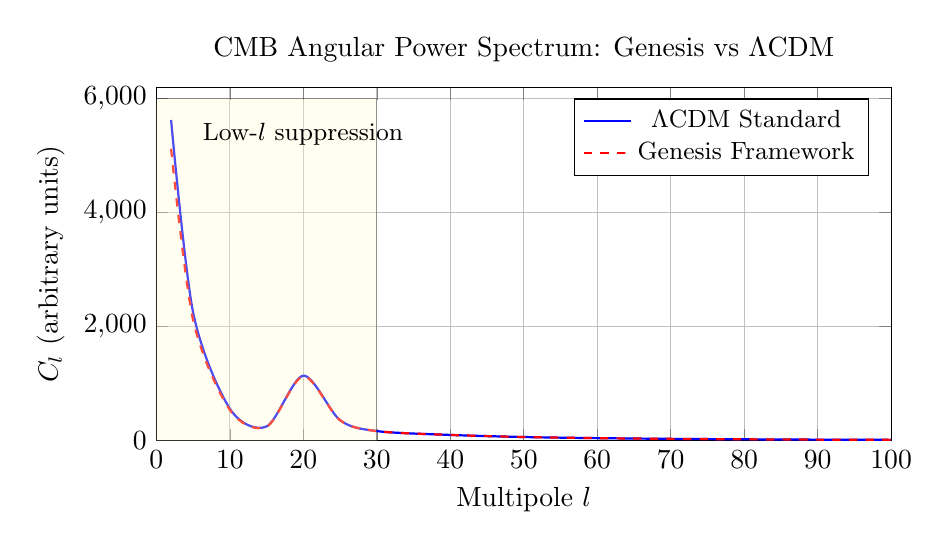
\begin{tikzpicture}
    \begin{axis}[
      width=0.9\textwidth,
      height=0.5\textwidth,
      title={CMB Angular Power Spectrum: Genesis vs $\Lambda$CDM},
      xlabel={Multipole $l$},
      ylabel={$C_l$ (arbitrary units)},
      xmin=0, xmax=100,
      ymin=0,
      grid=major,
      legend pos=north east,
      legend style={font=\small},
    ]
    % LCDM power spectrum (simplified with acoustic peaks)
    \addplot[
      blue, thick, smooth,
    ] table[x=l, y=C_LCDM, col sep=comma] {
      l,C_LCDM
      2,5625.0
      5,2250.0
      10,562.5
      15,250.0
      20,1140.625
      25,360.0
      30,168.75
      40,101.390625
      50,64.8
      60,45.0
      70,32.653061224489797
      80,24.609375
      90,18.909465020576134
      100,14.88
    };
    \addlegendentry{$\Lambda$CDM Standard}

    % Genesis power spectrum with low-l suppression
    \addplot[
      red, thick, dashed, smooth,
    ] table[x=l, y=C_Genesis, col sep=comma] {
      l,C_Genesis
      2,5120.338086
      5,2116.405898
      10,540.173664
      15,245.017969
      20,1129.869869
      25,358.704722
      30,168.428594
      40,101.253472
      50,64.742394
      60,45.038306
      70,32.683766
      80,24.634815
      90,18.931313
      100,14.899040
    };
    \addlegendentry{Genesis Framework}

    % Highlight low-l region
    \draw[fill=yellow!20, opacity=0.3] (axis cs:0,0) rectangle (axis cs:30,6000);
    \node[anchor=south west] at (axis cs:5,5000) {\small Low-$l$ suppression};
    \end{axis}
  \end{tikzpicture}

  \vspace{0.5cm}

  % Fractional difference
  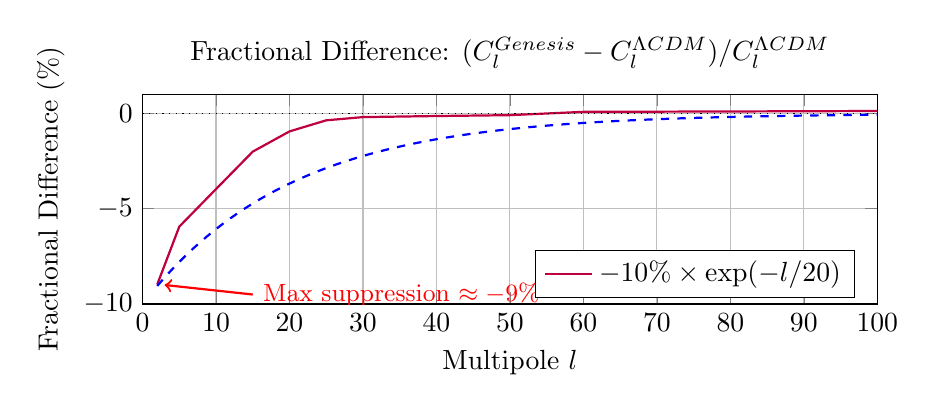
\begin{tikzpicture}
    \begin{axis}[
      width=0.9\textwidth,
      height=0.35\textwidth,
      title={Fractional Difference: $(C_l^{\text{Genesis}} - C_l^{\Lambda\text{CDM}}) / C_l^{\Lambda\text{CDM}}$},
      xlabel={Multipole $l$},
      ylabel={Fractional Difference (\%)},
      xmin=0, xmax=100,
      ymin=-10, ymax=1,
      grid=major,
      legend pos=south east,
    ]
    % Fractional difference data
    \addplot[
      mark=none,
      thick,
      color=purple,
    ] table[x=l, y=frac_diff, col sep=comma] {
      l,frac_diff
      2,-8.974
      5,-5.938
      10,-3.967
      15,-2.003
      20,-0.943
      25,-0.360
      30,-0.191
      40,-0.135
      50,-0.089
      60,0.085
      70,0.094
      80,0.104
      90,0.116
      100,0.128
    };

    % Theoretical suppression factor
    \addplot[
      blue, dashed, thick,
      domain=2:100,
      samples=100,
    ] {-10*exp(-x/20)};
    \addlegendentry{$-10\% \times \exp(-l/20)$}

    % Zero line
    \addplot[black, dotted] coordinates {(0,0) (100,0)};

    % Highlight max suppression at l ~ 2-5
    \draw[<-, thick, red] (axis cs:3,-9) -- (axis cs:15,-9.5) node[right] {\small Max suppression $\approx -9\%$};
    \end{axis}
  \end{tikzpicture}

  \caption{%
    \textbf{CMB angular power spectrum low-$l$ suppression in Genesis Framework.}
    \textit{Top}: Comparison of $\Lambda$CDM standard power spectrum (blue solid) with Genesis prediction (red dashed).
    Genesis nodespace structure suppresses power at low multipoles ($l < 30$) via
    $C_l^{\text{Genesis}} = C_l^{\Lambda\text{CDM}} \left(1 - \epsilon \exp(-l/l_0)\right)$
    with $\epsilon = 0.1$, $l_0 = 20$.
    Yellow shaded region highlights low-$l$ suppression zone.
    \textit{Bottom}: Fractional difference showing maximum $\approx -9\%$ suppression at $l \sim 2$--5,
    decaying exponentially with purple curve matching theoretical prediction (blue dashed).
    This signature is testable with Planck and future CMB experiments.
  }
  \label{fig:cmb-lowl-suppression}
\end{figure}

%==============================================================================
